%%%%%%%%%%%%%%%%%%%%%%%%%%%%%%%%%%%%%%%%%
% Structured General Purpose Assignment
% LaTeX Template
%
% This template has been downloaded from:
% http://www.latextemplates.com
%
% Original author:
% Ted Pavlic (http://www.tedpavlic.com)
%
% Note:
% The \lipsum[#] commands throughout this template generate dummy text
% to fill the template out. These commands should all be removed when
% writing assignment content.
%
%%%%%%%%%%%%%%%%%%%%%%%%%%%%%%%%%%%%%%%%%

%----------------------------------------------------------------------------------------
%	PACKAGES AND OTHER DOCUMENT CONFIGURATIONS
%----------------------------------------------------------------------------------------

\documentclass{article}

\usepackage{multirow}
\usepackage{amssymb}
\usepackage[fleqn]{amsmath}
\usepackage{url}

\usepackage{fancyhdr} % Required for custom headers
\usepackage{lastpage} % Required to determine the last page for the footer
\usepackage{extramarks} % Required for headers and footers
\usepackage{graphicx} % Required to insert images
\usepackage{lipsum} % Used for inserting dummy 'Lorem ipsum' text into the template

% Margins
\topmargin=-0.45in
\evensidemargin=0in
\oddsidemargin=0in
\textwidth=6.5in
\textheight=9.0in
\headsep=0.25in

\linespread{1.1} % Line spacing

% Set up the header and footer
\pagestyle{fancy}
\lhead{\hmwkAuthorName} % Top left header
\chead{\hmwkClass\ : \hmwkTitle} % Top center header
\rhead{\firstxmark} % Top right header
\lfoot{\lastxmark} % Bottom left footer
\cfoot{} % Bottom center footer
\rfoot{Page\ \thepage\ of\ \pageref{LastPage}} % Bottom right footer
\renewcommand\headrulewidth{0.4pt} % Size of the header rule
\renewcommand\footrulewidth{0.4pt} % Size of the footer rule

\setlength\parindent{0pt} % Removes all indentation from paragraphs

%----------------------------------------------------------------------------------------
%	DOCUMENT STRUCTURE COMMANDS
%	Skip this unless you know what you're doing
%----------------------------------------------------------------------------------------

% Header and footer for when a page split occurs within a problem environment
\newcommand{\enterProblemHeader}[1]{
\nobreak\extramarks{#1}{#1 continued on next page\ldots}\nobreak
\nobreak\extramarks{#1 (continued)}{#1 continued on next page\ldots}\nobreak
}

% Header and footer for when a page split occurs between problem environments
\newcommand{\exitProblemHeader}[1]{
\nobreak\extramarks{#1 (continued)}{#1 continued on next page\ldots}\nobreak
\nobreak\extramarks{#1}{}\nobreak
}

\setcounter{secnumdepth}{0} % Removes default section numbers
\newcounter{homeworkProblemCounter} % Creates a counter to keep track of the number of problems

\newcommand{\homeworkProblemName}{}
\newenvironment{homeworkProblem}[1][Problem \arabic{homeworkProblemCounter}]{ % Makes a new environment called homeworkProblem which takes 1 argument (custom name) but the default is "Problem #"
\stepcounter{homeworkProblemCounter} % Increase counter for number of problems
\renewcommand{\homeworkProblemName}{#1} % Assign \homeworkProblemName the name of the problem
\section{\homeworkProblemName} % Make a section in the document with the custom problem count
\enterProblemHeader{\homeworkProblemName} % Header and footer within the environment
}{
\exitProblemHeader{\homeworkProblemName} % Header and footer after the environment
}

\newcommand{\problemAnswer}[1]{ % Defines the problem answer command with the content as the only argument
\noindent\framebox[\columnwidth][c]{\begin{minipage}{0.98\columnwidth}#1\end{minipage}} % Makes the box around the problem answer and puts the content inside
}

\newcommand{\homeworkSectionName}{}
\newenvironment{homeworkSection}[1]{ % New environment for sections within homework problems, takes 1 argument - the name of the section
\renewcommand{\homeworkSectionName}{#1} % Assign \homeworkSectionName to the name of the section from the environment argument
\subsection{\homeworkSectionName} % Make a subsection with the custom name of the subsection
\enterProblemHeader{\homeworkProblemName\ [\homeworkSectionName]} % Header and footer within the environment
}{
\enterProblemHeader{\homeworkProblemName} % Header and footer after the environment
}

%----------------------------------------------------------------------------------------
%	NAME AND CLASS SECTION
%----------------------------------------------------------------------------------------


%----------------------------------------------------------------------------------------
%	TITLE PAGE
%----------------------------------------------------------------------------------------

\title{
\vspace{2in}
\textmd{\textbf{\hmwkClass:\ \hmwkTitle}}\\
\normalsize\vspace{0.1in}\small{Due\ on\ \hmwkDueDate}\\
\vspace{3in}
}

\author{\textbf{\hmwkAuthorName}}
\date{} % Insert date here if you want it to appear below your name



\usepackage{clrscode}
\usepackage{enumerate}
\newcommand{\hmwkTitle}{Assignment\ \#7} % Assignment title
\newcommand{\hmwkDueDate}{April\ 30,\ 2016} % Due date
\newcommand{\hmwkClass}{Algorithms} % Course/class
\newcommand{\hmwkAuthorName}{Zhaoyang Li (2014013432)} % Your name
%----------------------------------------------------------------------------------------

\begin{document}

\maketitle

%----------------------------------------------------------------------------------------
%	TABLE OF CONTENTS
%----------------------------------------------------------------------------------------

\setcounter{tocdepth}{1} % Uncomment this line if you don't want subsections listed in the ToC

\newpage
\tableofcontents
\newpage

%----------------------------------------------------------------------------------------
%	PROBLEM 1
%----------------------------------------------------------------------------------------


\begin{homeworkProblem}

CLRS Exercises 35.3-2,
Show that the decision version of the set-covering problem is NP-complete by reducing it from the vertex-cover problem.

\problemAnswer{
\paragraph{Part I} \proc{Set-Covering} $\in$ NP.

Trivially, for an given instance $(X,\mathcal{F},k)$ and its solution $S$, we can check if $S$ is a subset of $\mathcal{F}$ consisting of less than $k$ subsets of $X$, and whether $S$ covers $X$, in polynomial time.


\paragraph{Part II} Conversion

Given an instance of \proc{Vertex-Covering}, say $(V,E,j)$. Let $X=E, k=j$. For all vertexes $v_i\in V$, construct $E\supseteq E_i = \{e\in E: \exists v_j\in V s.t. (v_j, v_i) = e\}$. Let $\mathcal{F}=\{E_i\}$. Since $\mathcal{F}$ consists of subsets of $E$, the converted instance of \proc{Set-Covering} is valid. Such construction can be done in polynomial time.


\paragraph{PART III} Proof of correctness

(a) An instance of \proc{Vertex-Covering} is accepted \textbf{if} it's converted instance of \proc{Set-Covering} is accepted.

Suppose we have a solution $S$ to $(X,\mathcal(F),k)$, which covers $X$. $\forall S_i\in S$, there is a corresponding $v_i\in V$. Let the corresponding $v_i$'s form a set $V'$. We know that $|S|=|V'|=k=j$. Since $S$ covers $X$, it's obvious that $V'$ covers $(V,E)$.

(b) An instance of \proc{Vertex-Covering} is accepted \textbf{only if} it's converted instance of \proc{Set-Covering} is accepted.

Suppose we have a solution $S$ to $(V,E,j)$. There exists a corresponding $C\subseteq 2^E$ for each $v\in S$. Since $j=k$, $|C|\leq k$. $\forall x\in X$, it corresponds to an $e\in E$. Since $X$ is covered, $E$ is covered.

\paragraph{In conclusion,} \proc{Set-Covering}  $\leq_P$ \proc{Vertex-Covering}, and \proc{Set-Covering} $\in$ NP. Thus, \proc{Set-Covering} $\in$ NP-Complete.
}
\end{homeworkProblem}


%----------------------------------------------------------------------------------------
%	PROBLEM 2
%----------------------------------------------------------------------------------------


\begin{homeworkProblem}

CLRS Exercises 35.3-3,

Show how to implement \proc{Greedy-Set-Cover} in such a way that it runs in time $O\left(\sum_{S\in \mathcal{F}}|S|\right)$


\problemAnswer{
As far as I can see, to get such a low time complexity, we have to perform some space-time tradeoff, meaning that we need some spacial data structure.

Let's maintain an table $T_1$ of all the elements $S_i\in\mathcal{F}$, keeping them sorted by a $s_i=|\{x\in S_i : \text{not covered yet}\}|$.

Each time, we choose $S_j\in\mathcal{F}$ from $T_1$ with the maximum $s_j$, update all the $s_i$'s in $T_1$ (where "update" is always "decrease"), and repeat until $\forall j, s_j=0$.

$T_1$ is supposed to support \proc{Decrease-Key} and \proc{Find-Max} efficiently. I believe we can find some data structure to meet the requirements. Heaps, for instance.

Now, in order to update our $s_i$'s efficiently, we have to keep track of all $x_k\in X$: we need to know all the $S_i$'s $x_k$ is in, all the $s_i$'s in which $x_k$ counted. That requires tables mapping from $k$ to lists of $S_i$. In order to make locating quicker, we may want to add more internal links between all the tables.

Now let's describe our algorithm informally:

\begin{itemize}
\item Create $T_1$ mapping from $i$ to decreasingly-sorted integers, initially $|S_i|$. Create $T_2$ mapping from $i$ to $\{j:x_i\in S_j\}$. Let $C=\emptyset$.

\item Repeat until $\forall j, T_2(j)=0$: choose the maximum item in $T_1$ as $t$. Let $C=C\cup\{t\}$. For all $ x \in t$, for all $y\in T_2(x)$, $T_2(x)=T_2(x)\setminus\{y\}$, decrease the corresponding $T_1(y)$.

\item Return with $C$.
\end{itemize}
}
\end{homeworkProblem}

%----------------------------------------------------------------------------------------
%	PROBLEM 3
%----------------------------------------------------------------------------------------


\begin{homeworkProblem}

CLRS Problems 27-2,

Saving temporary space in matrix multiplication

\problemAnswer{
\subsection{a}
Modifications on the original \proc{P-Matrix-Multiply-Recursive} are listed as follows.

\begin{itemize}
\item add an initialization $\forall i, j, c_{ij} = 0$ outside, in parallel, in $\Theta(\lg n)$
\item add a \textbf{sync} statement after the 4th \textbf{spawn}
\item modify line 3 into $c_{11} = c_{11} + a_{11} \cdot b_{11}$
\end{itemize}

$T_\infty(n) = 2 T_\infty(n / 2) + \Theta(\lg n) = \Theta(n)$

\subsection{b}
Work: $T_1 = \Theta(n^3)$.
Span: $T_\infty = \Theta(n)$.

\subsection{c}
Parallelism: $T_1 / T_\infty = \Theta(n^2) = 1000^2 = 10^6$.

Though it's 10 times less than the original, since most parallel computers still have far fewer than 1 million processors, it's reasonable to conclude that there is no significant difference.
}
\end{homeworkProblem}



%----------------------------------------------------------------------------------------
%	PROBLEM 4
%----------------------------------------------------------------------------------------


\begin{homeworkProblem}

Implement multithreading versions of merge sort and quick sort with OpenMP.

\subsection{Implementation and environment}
\paragraph{Language} The C++ programming language
\paragraph{IDE} Visual Studio 2015
\paragraph{Compiling} MSVC2015 64bit Debug\footnote{Release with optimization disabled gives similar results.} with OpenMP support
\paragraph{OS} Windows 10 Education, Build 10586
\paragraph{Hardware} Intel Core i7-6600U @ 2.60GHz (2 Cores), RAM 16GB LPDDR3, Model ThinkPad X1 Carbon 20FB

\subsection{Verification of correctness}

Correctness is verified by comparing results given respectively by the algorithms, on randomly generated arrays. 100\% correctness.

\subsection{Timing}
Each number in the table below is an average over several different randomly generated arrays.
\begin{center}
\begin{tabular}{rrrrrr}
\hline
milliseconds&   Quick Single&	Quick Naive Multi&	Merge Single&	Merge Naive Multi&	Merge Multi\\
\hline
Array size 1e6&	1.90E+07&	1.35E+07&	4.16E+07&	3.29E+07&	2.09E+07\\
Array size 1e3& 	5081.22&	3929.41&	29941.2&	23651.2&	10828\\
\hline
\end{tabular}
\end{center}

Illustrated as follows.

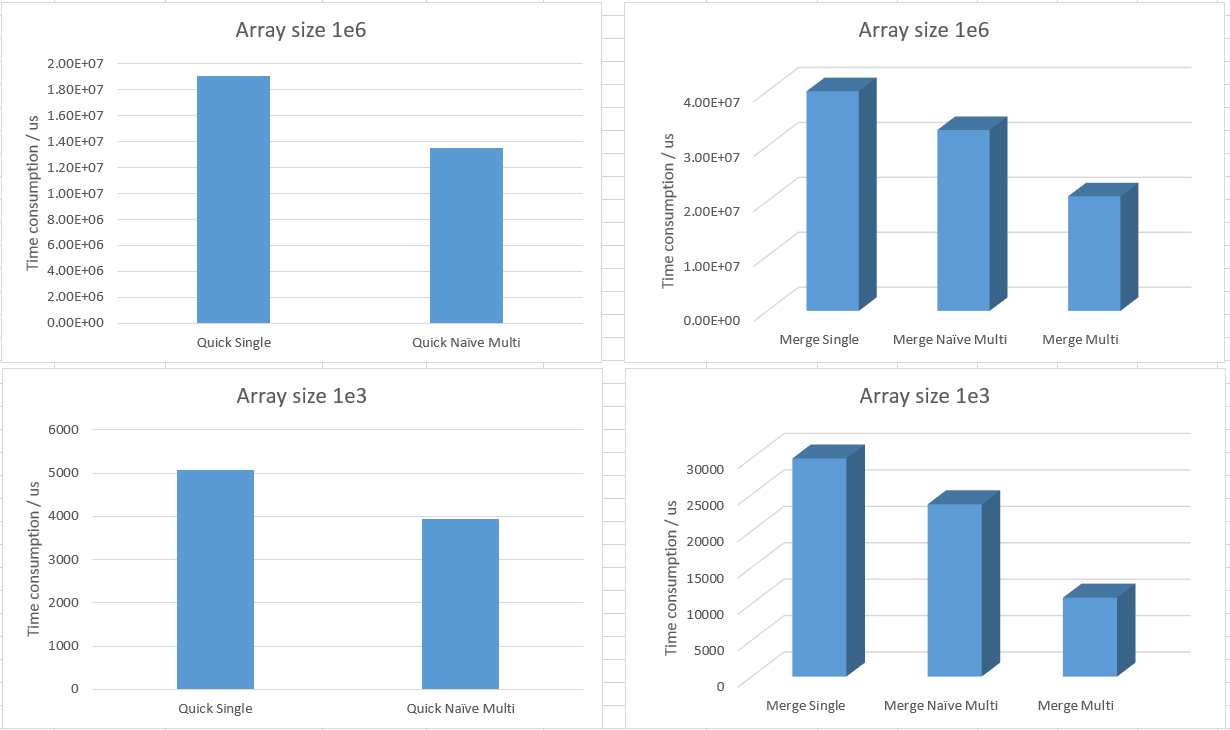
\includegraphics[width=1\columnwidth]{sort}

It can be concluded that multi-threading merge sort saves about 50\% of the running time, as is expected on a 2-core CPU. Naive multi-threading algorithms save 20\% to 30\%.


\end{homeworkProblem}




%----------------------------------------------------------------------------------------
%	PROBLEM 5
%----------------------------------------------------------------------------------------


\begin{homeworkProblem}

Implement GPU version of matrix multiplication with OpenCL or CUDA.

\subsection{Implementation and environment}
\paragraph{Language} The C++ programming language and the OpenCL C Language
\paragraph{IDE} Visual Studio 2015
\paragraph{Compiling} MSVC2015 64bit Release, Intel SDK for OpenCL Applications 6.0
\paragraph{OS} Windows 10 Education, Build 10586
\paragraph{Hardware} Intel Core i7-6600U @ 2.60GHz, GPU Intel HD Graphics 530, RAM 16GB LPDDR3, Model ThinkPad X1 Carbon 20FB

\subsection{Verification of correctness}

Correctness is verified by comparing results given respectively by the two implementations, on randomly generated matrices. 100\% correctness.

\subsection{Timing}
Each number in the table below is an average over several different randomly generated matrices.
\begin{center}
\begin{tabular}{rrr}
\hline
size& CPU/us& GPU/us\\
\hline
1& 	0.02& 	915.825378\\
2& 	0.05& 	867.252197\\
4& 	0.32& 	1014.651611\\
8& 	2.29& 	1159.98291\\
16& 	13.44& 	1057.659912\\
32& 	94& 	891.381287\\
64& 	850& 	938.103577\\
128& 	6000& 	1313.00354\\
256& 	52000& 	1707.822388\\
512& 	427000& 	5865.757813\\
1024& 	3.28E+06& 	36941.33203\\
2048& 	2.76E+07& 	236610.8594\\
4096& 	& 	1075285.25\\
8192& 	& 	7530680.5\\
\hline
\end{tabular}
\end{center}

Illustrated as follows.

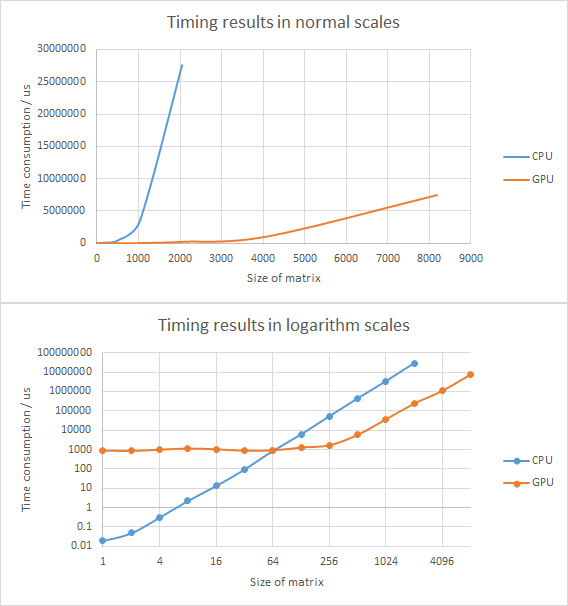
\includegraphics[width=.75\columnwidth]{matrix}

It can be concluded that for large matrices, GPU calculation is about 100 times faster. As the two lines on the log-log plot looks parallel with each other, we know that growth rate of running time on CPU and GPU are basically the same, which is $\Theta(n^3)$.

It's not expected that for small matrices, GPU has a fixed running time, regardless of the exact size of the matrix. I didn't look into details; a reasonable guess is that time spent on scheduling outweighs.

\end{homeworkProblem}

(End of all.)
%----------------------------------------------------------------------------------------

\end{document}
